 \documentclass{article}
\usepackage{graphicx,amsmath}
\usepackage[utf8]{inputenc}
\title{Generator \& Theory Working Group Chapter for CWP}
\author{
R. Boughezal (Argonne National Laboratory) \\ 
J.T. Childers (Argonne National Laboratory) \\
S. H{\"o}che (SLAC National Accelerator Laboratory) \\
O. Mattelaer (Universit\'e Catholique de Louvain) \\
J. McFayden (CERN)\\
S. Mrenna (Fermi National Accelerator Laboratory)\\
F. Petriello (Argonne National Laboratory \& Norwestern University)\\
S. Prestel (Fermi National Accelerator Laboratory)\\
C. Reuschle (Florida State University)}

\date{\today}

\def \Herwig {Herwig}
\def \Pythia {Pythia}
\def \mglo {MadGraph5\_aMC@NLO}
\def \mgnlo {MadGraph5\_aMC@NLO}
\graphicspath{{figures/}}

\begin{document}
\maketitle

\section{Introduction}

LHC experimental results continue to show excellent agreement with Standard Model predictions driving High Energy Physics into a new era of precision collider physics measurements. Theoretical predictions at the LHC and other colliders require perturbative calculations in Quantum Chromodynamics (QCD), the theory of the strong force that binds quarks and gluons into the colliding protons.  As a rough guideline to the required order in the QCD perturbative expansion, leading order (LO) only gets the order of magnitude of the result correct.  Next-to-leading order (NLO) gets results accurate to tens of percent.  Percent-level precision is possible at next-to-next-to-leading order (NNLO).  

Event generators use Monte Carlo methods to calculate the interaction cross-sections of LHC proton-proton collisions, and allow to interpret each unweighted Monte-Carlo sampling point as collision event in the measurement. This feature greatly alleviates a direct comparison between theory and experiment, and it makes event generators a necessity for interpreting measurements and identifying new physics beyond the Standard Model. 

The precision of LHC Run 2 analyses already rivals or exceeds the precision of theoretical predictions from NLO perturbative QCD \cite{AtlasZxs2017,AtlasWZxs2017}. As the LHC continues to break records in luminosity delivered and the High-Luminosity LHC (HL-LHC) comes online in 2025 experimental precision will continue to improve and the need for larger and larger simulated event samples will increase. The particle multiplicity per event continues to rise as well. These conditions drive an increase in the computing requirements of theoretical calculations and event generators. This chapter addresses plans for mitigating these increases and proposes solutions to ensure theory calculations and event generators are prepared to provide results in LHC Run 4 and beyond.

\subsection{Importance of Generators for LHC Experiments}

Event generators are the first step in the simulation chain of LHC experiments such as ATLAS and CMS. They calculate parton interaction cross-sections for LHC proton-proton interactions, then generate collision events based on these cross-sections. 
Figure~\ref{fig:atlas_grid_jobs_2016} shows the distribution of work performed by the ATLAS experiment on the grid in 2016 with 20\% going to event generation. ATLAS uses approximately 1.5 billion core-hours per year on the Grid and elsewhere. During the Run-1 (Run-2) MC production campaign, ATLAS generated 6.1 (12.5) billion events using 1.6 (91.4) CPU-time per event. 

There are two main contributing factors in the difference between Run-1 and Run-2 CPU consumption. During Run-1 the usage of Les Houches event (LHE) files~\cite{Alwall:2006yp,Andersen:2014efa} (produced with off-grid resources) was commonplace whereas this has largely been replaced with centralised LHE file production by ATLAS in Run-2. Also, in Run-2 higher precision calculations, for example using NLO merging, are more prevalent and such calculations naturally take up signifacntly more resources.


\begin{figure}
\centering
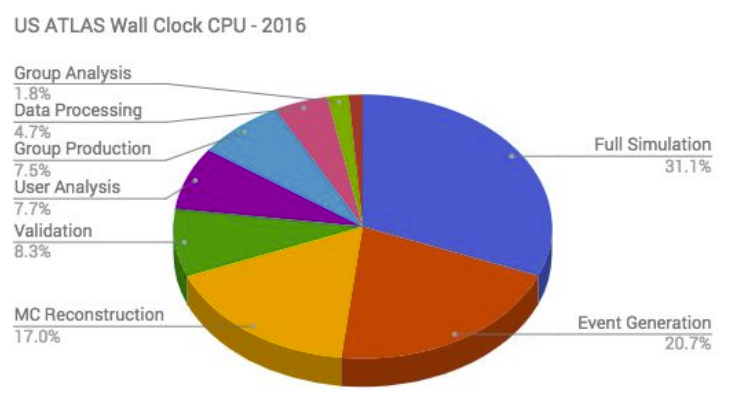
\includegraphics[width=0.7\textwidth]{atlas_grid_usage_2016}
\caption{Distribution of job types run by the ATLAS experiment in 2016.}
\label{fig:atlas_grid_jobs_2016}
\end{figure}

%\subsection{Challenges with current generators}

%\subsection{Characteristics of generators (dividing ME and PS, orders, etc) relevant for this discussion (not a detailed overview)}

\section{Current Landscape}

LHC experiments depend on many different physics event generators and theory calculations for both their similarities and their differences. The fact that theoretical approaches as well as implementations can vary offers an opportunity to validate and cross-check the predictions in a similar way that ATLAS and CMS provide systematic checks of experimental measurements. 

The following section reviews some of the more heavily used generators in LHC experiments and some leading edge theory calculations.

\subsection{Leading-Order Event Generators}
\label{ref:lo_generators}
Ever since the first detailed, phenomenological studies of
fragmentation by Feynman and Field \cite{Field:1977fa}, computer
simulations of ``events'' have played an increasingly important role
in understanding and validating the Standard Model.   
The roots of event generators begin
in the attempt to describe the non-perturbative hadronization process. 
With the acceptance of QCD, the perturbative evolution of partons was
added, yielding the parton shower description.   
The combination of leading order differential cross sections for 
the simplest Standard Model processes with the parton
shower and hadronization
model gave a good description of jet and weak boson physics.
To understand physics at hadron colliders, models of beam remnant
evolution (so-called underlying event models) were developed 
analogously to the first models of hadronization.
The challenging search for
the top quark at the Tevatron collider, and the inherent weakness of
the parton shower approach in predicting high-$p_T$ jets, led to
interfaces with tree-level matrix-element based predictions.
By the end of the Tevatron era, precise measurements of the top quark
cross section had necessitated the development of consistent NLO +
parton shower predictions.

At the start of the LHC era, two of the main event generators had
migrated to C++ code (Herwig++ and Pythia8) while a third had started
from the beginning in C++ (Sherpa).

In recent years, our ability to make predictions at NLO and NNLO has
increased by leaps and bounds.   Nonetheless, event generators are
still the main workhorses of LHC experiments, for direct physics
measurements, but also for the important tasks of
estimating trigger rates, occupancy, detector performance, etc.
Event generator predictions are used almost exclusively to describe
jet physics.    Many exotic physics scenarios beyond the Standard
Model can also be studied with event generators.
However, as a shift has been made to making matrix element based
predictions, event generators take on the role of handling 
the matching/merging of these predictions with the parton shower,
underlying event, hadronization, etc. In any event, lowest-order 
event generators remain a crucial part of high-energy-physics
computing.   Besides modeling hadronization in general, they are
needed for a detailed description of pile-up, minimum bias events,
the underlying event, and jet structure and sub-structure.

To give an example, the modeling of hadronization, perturbative QCD
and soft QCD effects dominate the uncertainty on the top quark mass derived
from data \cite{Khachatryan:2015hba} and are a significant part of
the uncertainty on the $W$ boson mass \cite{Aaboud:2017svj}.
Data-driven pile-up modelling needs to be validated and cross-checked 
with event generators (see e.g.~\cite{TheATLAScollaboration:2013pia}), 
theoretical uncertainties on the (sub-)structure of jets need to be 
assessed by parton showering~\cite{Bellm:2016rhh,Mrenna:2016sih,Bothmann:2016nao} and 
the effects of high-jet-multiplicity background and signal events 
must be modeled using multi-jet-merged calculations \cite{Catani:2001cc,Lonnblad:2001iq,Krauss:2002up,Mrenna:2003if,Mangano:2006rw,
  Alwall:2007fs,Hoeche:2009rj,Hamilton:2010wh,Hoeche:2012yf,Platzer:2012bs,
  Lonnblad:2012ix,Lonnblad:2012ng,Frederix:2012ps}. 

As another example, the simulation of pile-up events with event generators requires detailed models
of how the total proton-proton scattering cross section is distributed over
phase-space, and how different scattering processes (elastic scattering, 
diffractive scattering producing rapidity gaps, single- or multi-parton 
scattering) compete for the available phase space. These processes can
yield any number of detectable particles, with rare events containing 
a very large number of particles. The event generator model of pile-up-like
scatterings needs to avoid and bias like the bias that is e.g.\ introduced 
by cuts that are necessary to avoid singularities in perturbative
scattering calculations. This then means that a simultaneous integration of
processes with cross sections differing by many orders of magnitude is
necessary. In turn, this requires the generation of very large samples of
phase-space points. Currently, high-throughput computing is used to address this
problem. 

Another computational frontier of leading-order event generators is the 
generation of perturbative variations that allow to assess the uncertainties
of the calculations. This includes both uncertainties in the modelling of
the hardest scattering that produces the partonic seeds of jets as well as
uncertainties in the evolution of partons into jets of hadrons. Both of these
facets have recently seen a move away from schemes to produce individual
uncorrelated variations based on high-throughput computation towards producing
statistically correlated systematic variations on-the-fly in a single 
event-generator run~\cite{Bellm:2016rhh,Mrenna:2016sih,Bothmann:2016nao}. The 
latter means that automated uncertainty estimates might
become amenable to high-performance computing in the near future.

Finally, the omnipresence of matching- and merging approaches to 
enable an accurate modeling of multi-jet final states (for both
signal- and background processes) has shifted much of the computational
challenges of modern event-generator calculations to the production of
fixed-order multi-parton scattering events. The phase space in which 
parton-showering is allowed to produce additional partons is severely 
restricted by matching/merging. Thus, for matched/merged calculations, the 
efficiency of the calculation is almost directly inherited from the
efficiency of the fixed-order (LO, NLO, \dots) calculation,
%~\cite{Mcfayden:2016}
such that the bottlenecks 
described in Section 2.2 impact the event generator calculation as well.
An example for the capabilities of modern tree-level event generators
is given in Tab~\ref{tab:lo_gen_perf}.
\begin{table}
  \begin{center}
  \begin{tabular}{lcccc}
    \hline
    Process & $W^-$+0j & $W^-$+1j & $W^-$+2j & $W^-$+3j \\\hline
%    Processes (mapped) & 1 (1) & 3 (3) & 18 (42) & 28 (68) \\
    RAM Usage & $<$1MB & $<$1MB & 1MB & 2 MB \\
    Initialization time & $<$1s & $<$1s & $<$1s & 2s \\
    Startup time & $<$1s & $<$1s & $<$1s & $<$1s \\
    Integration time & 8s & 2m 4s & 22m 8s & 2h 3m \\
    MC uncertainty [\%] & 0.18 & 0.14 & 0.25 & 0.44 \\
    \hline\\[1mm]
    \hline
    Process & $W^-$+4j & $W^-$+5j & $W^-$+6j & $W^-$+7j \\\hline
%    Processes (mapped) & 88 (324) & 116 (436) & 280 (1332) & 344 (1648) \\
    RAM Usage & 23 MB & 81 MB & 435 MB & 1.51 GB \\
    Initialization time & 33s & 3m 17s & 51m 52s & 6h 50m \\
    Startup time & $<$1s & $<$1s & 2s & 12s \\
    Integration time & 1d 5h & 6d 23h & 32d 19h & 64d 15h \\
    MC uncertainty [\%] & 0.66 & 0.78 & 1.29 & 2.70 \\
    \hline
  \end{tabular}
  \caption{Example performance measures for the computation of $pp\to W^-+n$-jets production at $\mathcal{O}(\alpha^2\alpha_s^n)$. 
    The center-of-mass energy is 13~TeV and jets are
    defined as $p_{T,j}>30$~GeV, $|y_j|<4.5$. All partonic channels are included
    in the calculation, and the CKM matrix is chosen to be diagonal.
    Numbers are generated on a dual 18-core Intel$^\text{\textregistered}$
    Xeon$^\text{\textregistered}$ 2.30GHz CPU. Integration times are cumulative for all MPI ranks in the parallel calculation.
    \label{tab:lo_gen_perf}}
  \end{center}
\end{table}
Note that a staged approach of pre-tabulating and storing fixed-order results 
before showering, as e.g.\ used in the 
\textsc{MadGraph5\_aMC@NLO} + \textsc{Pythia} or 
\textsc{Alpgen} + \textsc{Pythia} event-generation chain, can leads to 
computational overhead since certain pieces of the fixed-order calculation 
(i.e.~splitting histories) have to be reconstructed at shower run-time to 
guarantee a consistent combination. This overhead can become significant
at high parton multiplicity, but may be amendable to speed gains from
high-performance computing. The approach of generating fixed-order
results and showering simultaneously also suffers from computational 
challenges, as it leads to increased executable size and the loss of 
information about the partonic scattering event. It is therefore obvious
clear that developments that make fixed-order calculations amenable to 
high-performance gains alone will not improve the speed and efficiency of 
matched/merged event generator calculations, Instead, developments in 
fixed-order parts as well as showers (and how they are used to enable 
matching/merging) have to go hand-in-hand with the integration of codes to
allow for maximal computational gain.

\subsection{Next-to-Leading Order Event Generators}

Calculations and event simulation at NLO in perturbative QCD are used both 
for direct comparison with experimental data that are corrected to the 
parton level, and as an input to particle-level event simulation.
At the tree level, calculations have long been performed completely automatically 
using programs like Alpgen \cite{Mangano:2002ea}, Amegic \cite{Krauss:2001iv}, 
Comix \cite{Gleisberg:2008fv}, CompHEP \cite{Boos:2004kh}, HELAC \cite{Kanaki:2000ey}, 
MadGraph \cite{Alwall:2011uj} and Whizard \cite{Kilian:2007gr}.
At the next-to-leading order, such a level of automation required two main ingredients: 
The implementation of known generic methods to perform the subtraction of infrared 
singularities and the automated computation of one-loop amplitudes. 

The calculation of virtual corrections for processes with a large number
of hard, light jets in the final state has been one of the focal points 
in the past decades. The field received a boost from generalized unitarity 
\cite{Bern:1994cg,Bern:1994zx,Bern:1997sc}, which is used in this context
to determine one-loop amplitudes by decomposing them into known scalar 
one-loop integrals and rational coefficients determined from on-shell 
tree amplitudes, plus a rational piece \cite{Ossola:2006us,Forde:2007mi,
  Ellis:2007br,Ossola:2008xq,Ellis:2008ir,Peraro:2014cba,Hirschi:2016mdz}. A large number of programs have been 
developed that automate these methods~\cite{Berger:2008sj,Ellis:2008qc,Ellis:2009zw,Bevilacqua:2011xh,Hirschi:2011pa,Alwall:2014hca,Badger:2010nx,Cascioli:2011va,Cullen:2011kv,Fleischer:2011bi} based on library computing the scalar integral \cite{Ellis:2007qk,vanHameren:2010cp,Hahn:1998yk,Patel:2016fam,vanOldenborgh:1990yc} 
and that supplement well-established codes based on analytic calculations
\cite{MCFM,Campbell:2010ff,Campbell:2015qma} and on improved automated 
tensor reduction \cite{Denner:2005nn,Binoth:2005ff,Cullen:2011xs,Cullen:2014yla,
  Cascioli:2011va,Actis:2012qn}. A completely numerical approach exists \cite{Becker:2010ng,Becker:2011vg}. 
All these developments have brought about the construction of ever faster 
numerical programs for phenomenological applications. Monte-Carlo methods 
can be used to reduce the number of loop-evaluations when computing NLO computation \cite{Alwall:2014hca} allowing to have NLO computations not dominated by loop-computations. An example for the arising timing distribution
is shown in Table \ref{table:MG5NLO}. Despite all these advantages, NLO
computations typically require significantly more computing power
than their leading-order counterparts. In addition, the numerical methods
to evaluate NLO corrections can suffer from numerical instabilities, such that re-evaluation in higher precision arithmetics becomes necessary. In this case the computation can be slowed down significantly.

\begin{table}
  \begin{center}
    \begin{tabular}{lccc}
\hline
process & Virtual & Tree-Level & Subtraction \\
\hline\hline
$p p \to t \bar t$ & 18\% & 17\% & 37\% \\
$p p \to t  \bar t j$ & 35\% & 23\% & 38\% \\
$p p \to t  \bar t j j $ & 31\% & 32\% & 34\% \\
\hline
$p p \to W^+ W^- $ & 10\% & 20\% & 48\% \\
$p p \to W^+ W^- j$ & 15\% & 36\% & 36\% \\
$p p \to W^+ W^- j j$ & 35\% & 38\% & 23\% \\
\hline
$p p \to e^+ e- $ & 4\% & 14\% &  26\% \\
$p p \to e^+ e- j $ & 3\% & 51\% & 34\% \\
$p p \to e^+ e- j j$ & 14\% & 40\% & 31\% \\

\hline
    \end{tabular}
    \caption{\label{table:MG5NLO} Relative CPU time dedicated to the evaluation of the virtual matrix-element, of the tree-level matrix-element (Born and Real) and of the various subtraction terms. Numbers are computed with {\sc MadGraph5\_aMC@NLO}. The difference between 100\% and the sums of virtual, tree-level and subtraction is due to other parts of the code (like generating/writing events, computation of systematics, etc.)}
   \end{center}
\end{table} 

A major bottleneck is nowadays often found in the computation of 
real corrections and the corresponding infrared subtraction terms
\cite{Catani:1996vz,Catani:2002hc}.
The subtraction terms consist of color-correlated tree-level 
matrix elements multiplied by spin-dependent splitting operators, 
hence the aforementioned programs for leading order calculations 
are ideally suited for this part of the computation. Correspondingly,
infrared subtraction techniques have been implemented in various
general-purpose matrix element generators \cite{Gleisberg:2007md,
  Czakon:2009ss,Frederix:2008hu,Frederix:2010cj,Frederix:2009yq}.
Their reach is expanded sinificantly by parallel computing \cite{Hoche:2013zja,Bern:2013gka,Hoche:2016elu}, and it is expected
that this trend will continue in the future.


\subsection{NNLO Fixed-Order Calculations}

Achieving NNLO precision is an enormously difficult theoretical challenge.  Individual contributions to the expansion are separately divergent, necessitating regularization at intermediate stages.  It is also an enormous computational challenge.


These theoretical and computational challenges have received significant attention in the community  New methods have proven capable of providing the NNLO predictions needed to match the exacting experimental precision.  Those which have proven capable of handling the full complexity of $2 \to 2$ scattering with colored final states at the LHC are: antennae subtraction~\cite{GehrmannDeRidder:2005cm}; $N$-jettiness subtraction~\cite{Boughezal:2015dva,Gaunt:2015pea}; sector-improved residue subtraction~\cite{Czakon:2010td,Boughezal:2011jf}.  Together these techniques have made possible NNLO predictions for $W$+jet~\cite{Boughezal:2015dva}, $Z$+jet~\cite{Ridder:2015dxa,Boughezal:2015ded}, Higgs+jet~\cite{Boughezal:2015dra,Boughezal:2015aha,Chen:2014gva}, and $t\bar{t}$ production~\cite{Czakon:2013goa}, as well as partial results for di-jet production~\cite{Ridder:2013mf}.   We demonstrate the utility of these higher-order calculations using a result for the $Z$+jet process obtained using $N$-jettiness subtraction~\cite{Boughezal:2016yfp}.   The figure shows a plot for the $H_T$ distribution in the $Z$+jet process.  This observable provides an important control sample in the search for dark matter at colliders.  The data points as measured by the experimental collaborations are shown as points with error bars.  Theory predictions at NLO and NNLO are shown as red and blue bands respectively, where the bands denote an estimate of the residual theoretical error.  The NLO result falls below the measured data by nearly a factor of two, and fails to properly describe the distribution shape.  The NNLO prediction obtains both the correct normalization and shape.  More examples and a detailed discussion of the theoretical precision are given in Ref.~\cite{Boughezal:2016yfp}, but the message of this plot is clear: one simply cannot describe this important LHC data without a NNLO prediction.  

\begin{figure}
\centering
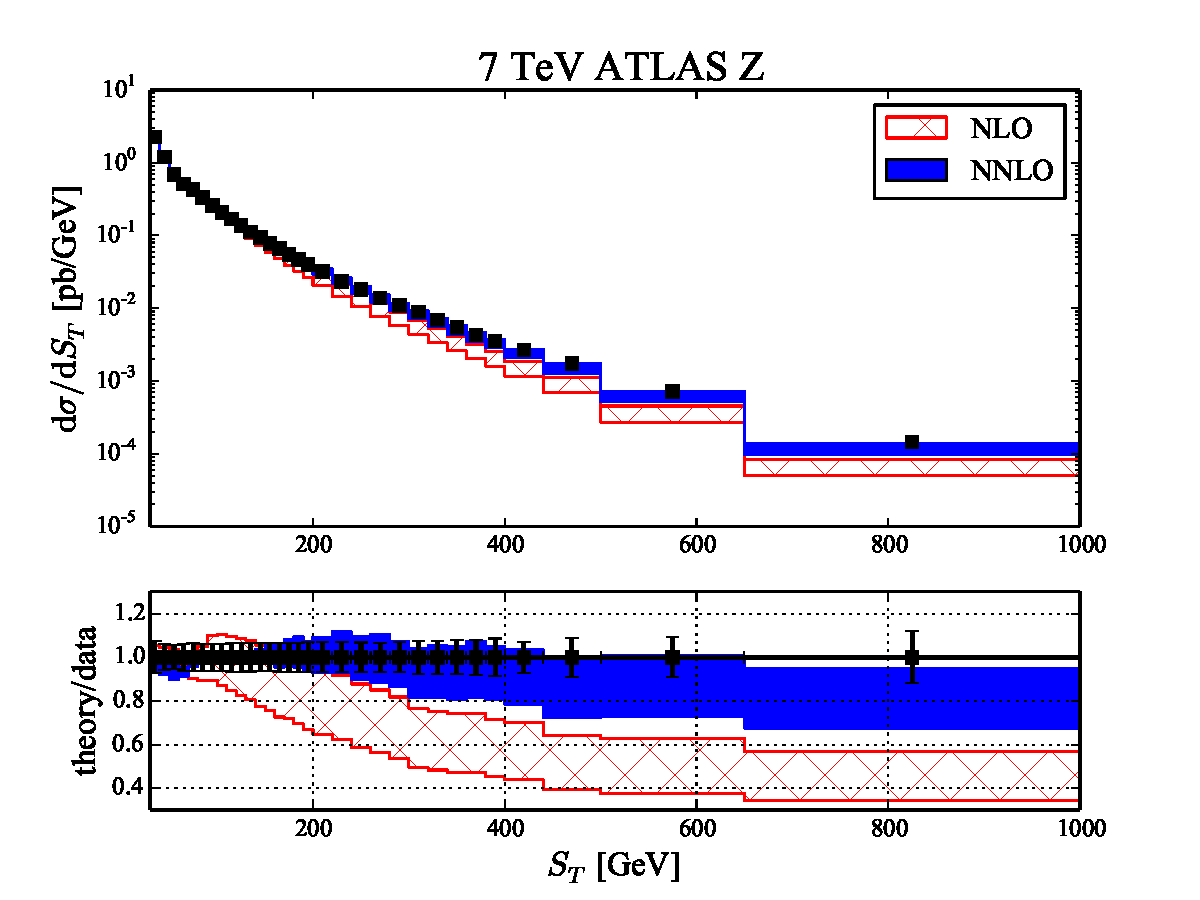
\includegraphics[width=3.21in]{ATLAS-Z-7TeV_HT}
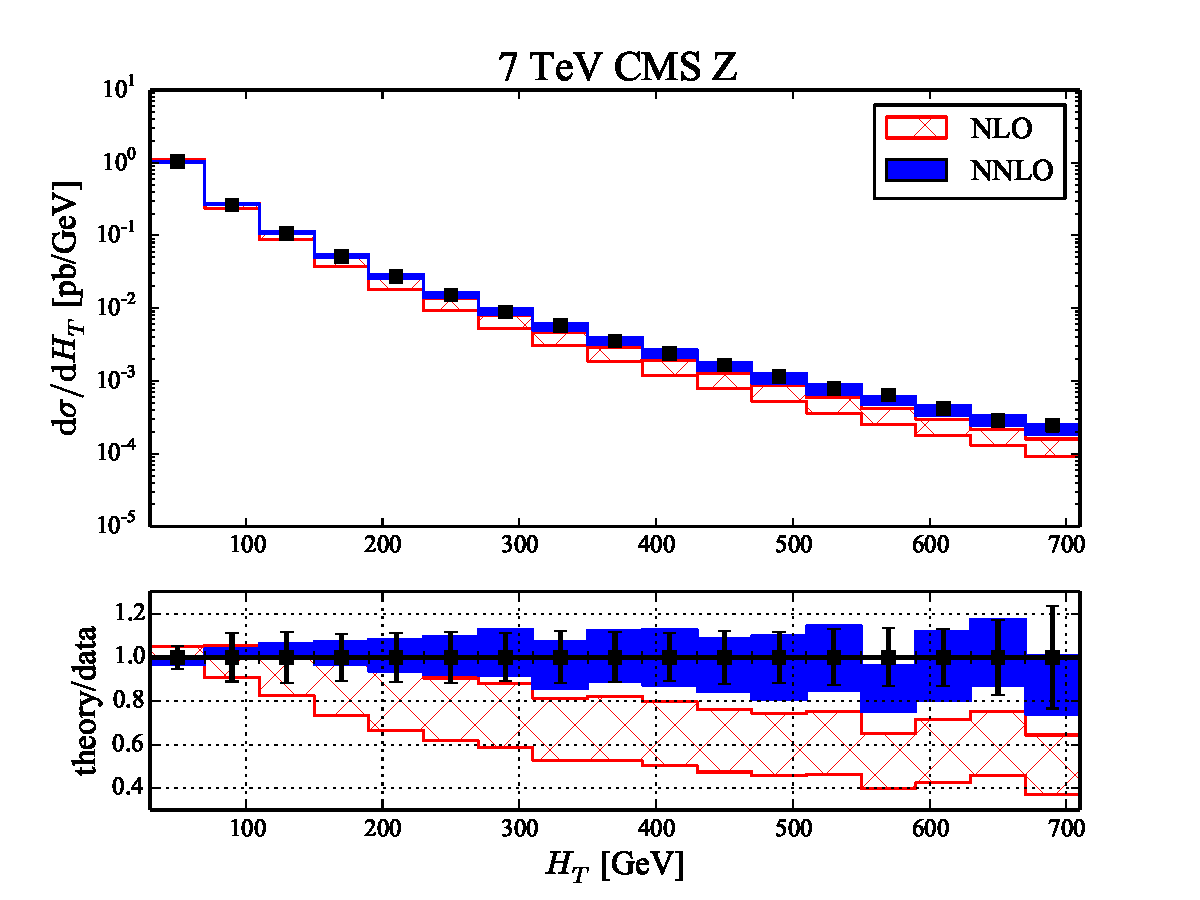
\includegraphics[width=3.21in]{CMS-Z-7TeV_HT}
\caption{Comparison of the $H_T$ distribution in the $Z$+jet process measured by ATLAS (left panel) and CMS (right panel) to theoretical predictions at NLO and NNLO.  The data points denote the experimental measurements with the reported errors, while the red and blue bands respectively denote the estimated NLO and NNLO theoretical errors.}
\label{fig:CMSZ}
\end{figure}


We discuss the computational aspects and challenges at NNLO using $N$-jettiness subtraction as an example.  The $N$-jettiness subtraction idea utilizes a novel computational approach that relies critically on parallel high-performance computing (HPC) systems.  The $N$-jettiness subtraction scheme achieves NNLO precision for LHC scattering processes by splitting the necessary integrations over the phase space of the $N$ final-state particles according to a resolution criterion on the $N$-jettiness event shape variable:
%
%\vspace{-.15in}
\begin{equation} \label{eq:PSsplit} 
\sigma_{{\rm NNLO}}=\int d\Omega \, \left[ \frac{{\rm d}\sigma_{{\rm NNLO}}}{{\rm d} {\cal T}_N} 
	\theta({\cal T}_N^{cut}-{\cal T}_N)
	+ \frac{{\rm d}\sigma_{{\rm NNLO}}}{{\rm d} {\cal T}_N} \theta({\cal T}_N-{\cal T}_N^{cut}) \right].
\end{equation} 
%
The $N$-jettiness variable ${\cal T}_N$ was defined in Ref.~\cite{Stewart:2010tn}.  For our purposes we note that it divides the phase space into an `above-cut' region (the second term in Eq.~\ref{eq:PSsplit}, where ${\cal T}_N>{\cal T}_N^{cut}$) which can be obtained from a simpler NLO calculation for $N+1$ jets.  The `below-cut' region (the first term in Eq.~\ref{eq:PSsplit}, where ${\cal T}_N<{\cal T}_N^{cut}$) can be obtained from an all-orders result in the strong coupling constant~\cite{Stewart:2009yx}.  A detailed discussion of how this technique is practically implemented was presented in the initial work.  The end result is the reduction of the number of required integrations to three: a computationally-simple below-cut integration, and two computationally-intensive above-cut integrations.  These integrations typically live in 10-15 dimensions and contain numerous peaks throughout phase space, and are approached with Monte-Carlo techniques such as the VEGAS algorithm~\cite{Lepage:1977sw}.

The primary computational challenge is that each integral in Eq.~(\ref{eq:PSsplit}) contains logarithms of the resolution 
parameter ${\cal T}_N^{cut}$ that cancel upon addition of all three terms.  Each separate term has up to ${\rm log}^4 ({\cal T}_N^{cut})$ dependence.  Since ${\cal T}_N^{cut}$ must be taken small for theoretical reasons, we must dig out the residual result from the numerical noise induced by the cancellation between large logarithms in the numerical integration.  The figure-of-merit to consider is the degree of cancellation between the above-cut and below-cut integrations.  In applications considered so far this ranges from 1 part in 10 to 1 part in 1000.   The desired numerical precision on the final result is sub-percent, implying that some of the separate integrals must be computed to $10^{-6}$ relative accuracy.  To reach this target for a Monte Carlo integration with a large number of dimensions requires an enormous number of integrand evaluations.  We split these between many threads, which must be coupled in order to use this information to appropriately refine the integration grid.  This explains the need for a massively parallel HPC resource.

The  $N$-jettiness subtraction method is a general theoretical framework that can be implemented in publicly available  codes for NLO calculations.  Several independent codes incorporating $N$-jettiness subtraction have been successfully run on the Mira supercomputer at the Argonne Leadership Computing Facility (ALCF)~\cite{Boughezal:2016wmq,Abelof:2016pby}.  These are written in a combination of Fortran77 and Fortran90.   All codes performs a Monte-Carlo integration of multi-dimensional integrands.  The many required integrand evaluations are the most computationally expensive part of the code, are parallelized using a hybrid MPI-OpenMP approach.  Reasonably good scaling up to the million-thread level is obtained on the Mira supercomputer at the ALCF.  As more complex scattering processes are studied, this scaling will become increasingly important.  

\subsection{Parton Showers at Higher Order}
Parton shower algorithms describing QCD and QED multiple radiation have been
a central ingredient of simulation programs for particle physics experiments
at the energy frontier~\cite{Webber:1986mc,Buckley:2011ms}. Invented about
three decades ago, they have undergone tremendous developments since then, 
with some of the most important steps being the introduction of QCD coherent evolution~\cite{Webber:1983if,Marchesini:1983bm,Marchesini:1987cf} and the 
incorporation of process-independent soft-gluon enhacement~\cite{Catani:1990rr}.

About a decade of work has been spent on matching~\cite{Frixione:2002ik,
  Hoeche:2011fd,Hamilton:2012rf,Hamilton:2013fea,Hoeche:2014aia,Hoche:2014dla}
and merging~\cite{Catani:2001cc,Lonnblad:2001iq,Krauss:2002up,Mangano:2006rw,
  Alwall:2007fs,Hoeche:2009rj,Hamilton:2010wh,Hoeche:2012yf,Platzer:2012bs,
  Lonnblad:2012ix,Lonnblad:2012ng,Frederix:2012ps} algorithms to include 
fixed-order higher-order corrections. More recently, the need for improved 
overall simulations triggered a resurgence of interest in improving 
parton-shower algorithms themselves. Several new parton showers have been 
constructed~\cite{Gieseke:2003rz,Sjostrand:2004ef,Schumann:2007mg,Dinsdale:2007mf,
  Winter:2007ye,Giele:2007di,Platzer:2009jq,Ritzmann:2012ca,Hoche:2015sya}, 
and the possibility of including next-to-leading order corrections into 
the evolution has been explored~\cite{Hartgring:2013jma,Li:2016yez,
  Hoche:2017iem,Hoche:2017hno,Nagy:2017ggp}. In addition, NLO splitting functions 
have been recomputed~\cite{Jadach:2011kc,Gituliar:2014eba}, with the aim 
to improve parton-shower simulations, and the dependence of NLO matching terms on the 
parton-shower evolution variable has been investigated~\cite{Jadach:2016zgk}.

While all these developments may lead to theoretically improved simulations rather soon,
they also require a significant increase in computation time for the generation
of each event. As a simple example, the implementation of next-to-leading order
accurate splitting functions in the parton shower effectively turns the previously
probabilistic simulation of the parton branching process into a true NLO
calculation. The occurrence of negative weights for the splitting kernels
is characteristic and leads to additional weight fluctuations in the overall 
simulation that have to be compensated by a higher number of generated events,
while each event also comes at an additional computational cost. This situation 
is very much alike to fixed-order perturbation theory.

%\subsection{Current Performance Measures}

%Table~\ref{tab:gen_perf} shows the average time (in seconds) it takes to generate one ttbar event on the Grid. The averages include number of sites to make them representative. 

%\begin{table}
%\centering
%\caption{My caption}
%\label{tab:gen_perf}
%\begin{tabular}{l|c|c}
%generator & process & seconds per event \\
%\hline
%Sherpa & ttbar all-hadronic & $49\pm13$ \\
%Pythia8 & ttbar & $0.012\pm0.005$ \\
%Powheg+Pythia & ttbar & $82\times10^{-6}\pm24\times10^{-6}$ \\
%MadGraph+Pythia & ttbar & $0.0012\pm0.0005$ \\
%aMC@NLO+Pythia & ttbar & $0.014\pm0.004$ 
%\end{tabular}
%\end{table}

%\begin{itemize}
%\item events/core-hour ?
%\item  LO vs NLO ? NNLO?
%\item Integration vs Generation ?
%\item Production time spent by the experiments ?
%\end{itemize}

\section{Future Strategies}

The following techniques will be investigated with the goal of increasing the precision of generators needed for analyses of the HL-LHC while aiming to reduce our computing requirements.

%\subsection{Evolutionary Techniques}

\subsection{Scalable Adaptive Monte-Carlo Integrators}

As generators move to higher orders in perturbative QCD and the HL-LHC probes higher multiplicity processes, the time needed to integrate the interaction cross-section becomes prohibitively large on a single CPU core. Parallel processing becomes a requirement and being able to scale on a supercomputer enables ever more aggressive analyses. 

Existing generators were not developed in the mulit-core age that has become the industry standard in the past five years and therefore parallel processing was added after frameworks had largely been implemented. This leads to meager performance improvements when running in parallel, especially when running in parallel across many compute nodes of a supercomputer. Work has been done to improve scalability of existing generators such as Sherpa and Alpgen~\cite{AlpgenScaling2017}. 

In the case of advanced frameworks such as MadGraph and Sherpa, the architecture of the framework was not designed to take advantage of highly parallel computers and maintain high CPU and memory efficiency. The development of new scalable adaptive Monte-Carlo integrators that can be used by existing frameworks would be a big step toward addressing HL-LHC computing requirements. In the US, the DOE is planning to deploy supercomputers over the next five years that will increase the scientific computing capacity by a factor of 200. Developing algorithms that target these machines will offload computation from Grid resources and will in general lead to the development of better algorithms.

% The full phase-space integral for multi-particle interactions factorizes into lower-dimensional integrals corresponding to $2\rightarrow2$-scattering and $1\rightarrow2$-decay processes. This can be used as a guiding principle to create integrators for high-multiplicity processes. The factorization is typically performed for each tree graph in each partonic channel in order to map out all known peaks of the integrand. Interferences between the Feynman graphs can be dealt with using the multi-channel method~\cite{Kleiss:1994qy} and the single-diagram enhanced integration technique~\cite{Maltoni:2002qb}. The latter may be well suited for parallelization if the integrand can be divided into a large number of graphs, which is always the case in high-multiplicity processes.

% Creating a new common integration tool which scales from laptop to HPC is a goal of the Generator \& Theory community. Such a tool will require evaluating the existing methods and studying the latest Monte-Carlo and quasi-Monte-Carlo techniques. The goal should be to introduce more parallelism and provide intelligence to determine at which scale different methods may lead to faster results for a target accuracy. Such a tool should use standard libraries that are compatible on clusters and HPCs, such as MPI or OpenMP (the latest version of which can target both CPUs and GPUs). It must be compatible with existing generator frameworks for use as a plugin.


\subsection{Reweighting of Event Samples}

Re-weighting method consists to attach to a given partonic events a new weight corresponding to a new theory. Those new weights allow to predict accurately (up to statistical precision) all the differential distributions at parton-level and to perform a single detector simulation for all the models under consideration.

Different types of re-weighting exist. First there is the reweighting mentioned in Sec.~\ref{ref:lo_generators}, which relates to the estimation of the theoretical uncertainties of a simulation. 
Second the same techniques can be used to accomodate BSM re-weighting for both LO \cite{Gainer:2014bta,Baglio:2014uba,Kalinowski:2016qcd,Mattelaer:2016gcx} and  NLO event samples, both approximatively \cite{Alioli:2010xd,REPOLO} and exactly \cite{Mattelaer:2016gcx}.

At LO accuracy the new weight ($W_{new}$) can be easily obtained from the original one ($W_{orig}$) by simply multiplying it by the ratio of the matrix-elements estimated on that event for both models (noted respectively $|M_{orig}|^2$ and $|M_{new}|^2$):
\begin{equation}\label{me_re-weighting}
W_{new} = \frac{|M_{new}|^2}{|M_{orig}|^2}W_{orig}.
\end{equation}
While at NLO, one needs to track the dependence in the various event and counter-event and reweight by the associated matrix-element.

A few remarks are in order regarding the range of validity of this method. First, even if the method returns the correct weight, it requires that the event sampling related to $W_{orig}$ covers appropriately the phase-space for the new theory. In particular, $W_{orig}$ must be non-zero in all regions where $W_{new}$ is non-vanishing. Though obvious, this requirement is in fact the most important and critical one. 
In other words, the phase-space where the new theoretical hypothesis contributes should be a subset of the original one. For example, re-weighing can not be used for scanning over different mass values of the final state particles\footnote{For intermediate particle a small variation of the mass --order of the width-- is reasonable.}, yet it is typically well-suited for probing different types of spin and/or coupling structures.

Second, the parton-level configuration feeder to parton-shower programs not only depends of the four-momenta but also of additional information, which is commonly encoded in the Les Houches Event File (LHEF) \cite{Alwall:2006yp,Andersen:2014efa}. Consequently, re-weighting  by an hypothesis that does not preserve such  additional information is not accurate. In general, such informations are related to:

\begin{itemize}
\item {\bf Helicity:} The helicity state of the external states of a parton-level event is optional in the LHEF convention, yet some programs (e.g. \cite{Meade:2007js}) use this information to decay the heavy state with an approximated spin-correlation matrix. \cite{Mattelaer:2016gcx,Artoisenet:2012st}
proposes a dedicated re-weihting method in this case to fix such issue.

\item {\bf Color-flow:} A second piece of information presented in the LHEF is the color assignment in the large $N_c$ limit. This information is used as the starting point for the dipole emission of the parton shower and therefore determines the result of the QCD evolution  and hadronisation.  Such information is untouched by the re-weigthing limiting the validity of the method. 

\item {\bf Internal resonances:} In presence of on-shell propagators, the associated internal particle is written in the LHEF. This is used by the parton-shower program to guarantee that the associated invariant mass is preserved during the re-shuffling procedure intrinsic to the showering process. Consequently, modifying the mass/width of internal propagator should be done with caution since it can impact the parton-shower behaviour. This information can not be corrected via a re-weighting formula, as it links in a non-trivial way short-distance with long-distance physics.
\end{itemize}

Even with such limitation the application of such re-weighting will allow to decrease by huge factor the time spent on the generation of BSM samples.
  

\bibliographystyle{abbrv}
\bibliography{main}

\end{document}
